\chapter{Predicting the unbiased MET Distribution at Higher Luminosity}
\section{Objective}
Our goal is to empirically reconstruct the unbiased CELL MET distribution using ZeroBias HLT noalg L1XE30 and HLT noalg L1XE50 data. 
We want to use this data to determine the CELL MET distribution as a function of $\mu$.
Because the ZeroBias events only allow us to go up to about $80$ GeV, we use the \texttt{HLTnoalg\_L1XExx} triggered events in order to extend to higher MET.
We correct the \texttt{HLTnoalg\_L1XExx} data using the efficiency curves determined from lower threshold triggers.
While performing this correction, it was important to propagate the errors due to the determination in the efficiency, and those due to statistical uncertainties.
Performing the reconstruction involved several steps:
\begin{enumerate}
        \item compute the efficiency of $L1>30$GeV for \texttt{HLT\_ZB\_L1ZB} data as a function of CELL MET
        \item correct the \texttt{HLT\_ZB\_L1XE30} data back to the \texttt{HLT\_ZB\_L1ZB} distribution by multiplying by the prescale and dividing by the efficiency. 
        \item compute the efficiency of $L1>50GeV$ for \texttt{HLT\_ZB\_L1XE30} data as a function of CELL MET
        \item correct the \texttt{HLT\_ZB\_L1XE50} data back to the \texttt{HLT\_ZB\_L1ZB} distribution by multiplying by the corresponding prescale, and dividing by both of the previously computed efficiencies. 
\end{enumerate}
For this project, we used the 2015, 2016 and 2017 combined \texttt{HLTnoalg\_L1ZB} , \texttt{HLTnoalg\_L1XE30} and \texttt{HLTnoalg\_L1XE50} data produced by Jonathan Burr on 11/17/2017 from the zerobias and JETM10 trees.
In addition, we removed the events from runs 330203, 331975 and 334487 because these events had large MET events without jets and the logbook says there were calorimeter noise problems in these runs. 

\section{Efficiency Fits}
It was necessary to come up with a model that could be used to fit to our efficiency data. To create this model, we assumed that the conditional distribution of the value of MET as determined by L1, given the value of MET as determined by CELL was a gaussian:
\begin{align}
		\mathbb{P}(X=x|Y) = \frac{1}{\sigma \sqrt{2\pi}} e^{-z^2/2\sigma^2}
\end{align}
Where we have defined:
\begin{align}
		z=y-(ax+b)
\end{align}
Then, in order to derive the expression for the model for the efficiency curves, we compute the probability that L1 determines as MET value higher than the value of the threshold. In order to do this, we integrate from the value of the threshold ($T$) to infinity:
\begin{align}
		\varepsilon(x)=\frac{1}{\sigma \sqrt{2\pi}}\int_{T}^{\infty}e^{-z^2/2\sigma^2}dz
\end{align}
One may manipulate this expression using properties of integration, probability density functions and gaussians in order to write an expression for the efficiency in terms of the error function:
\begin{align}
		\textrm{Erf}(z)=\frac{2}{\sqrt{\pi}}\int_0^{z}e^{-t^2}dt
\end{align}
Finally, the expression we get is:
\begin{align}
		\varepsilon(x)=\frac{1}{2}\left( 1+\textrm{Erf}\left( \frac{ax+b-T}{\sigma\sqrt{2}} \right) \right)
\end{align}
We performed this fit for the distribution of MET in $\mu$ bins of $0-10,\ldots,60-70$
\pagebreak
\begin{figure}[h]
		\centering
		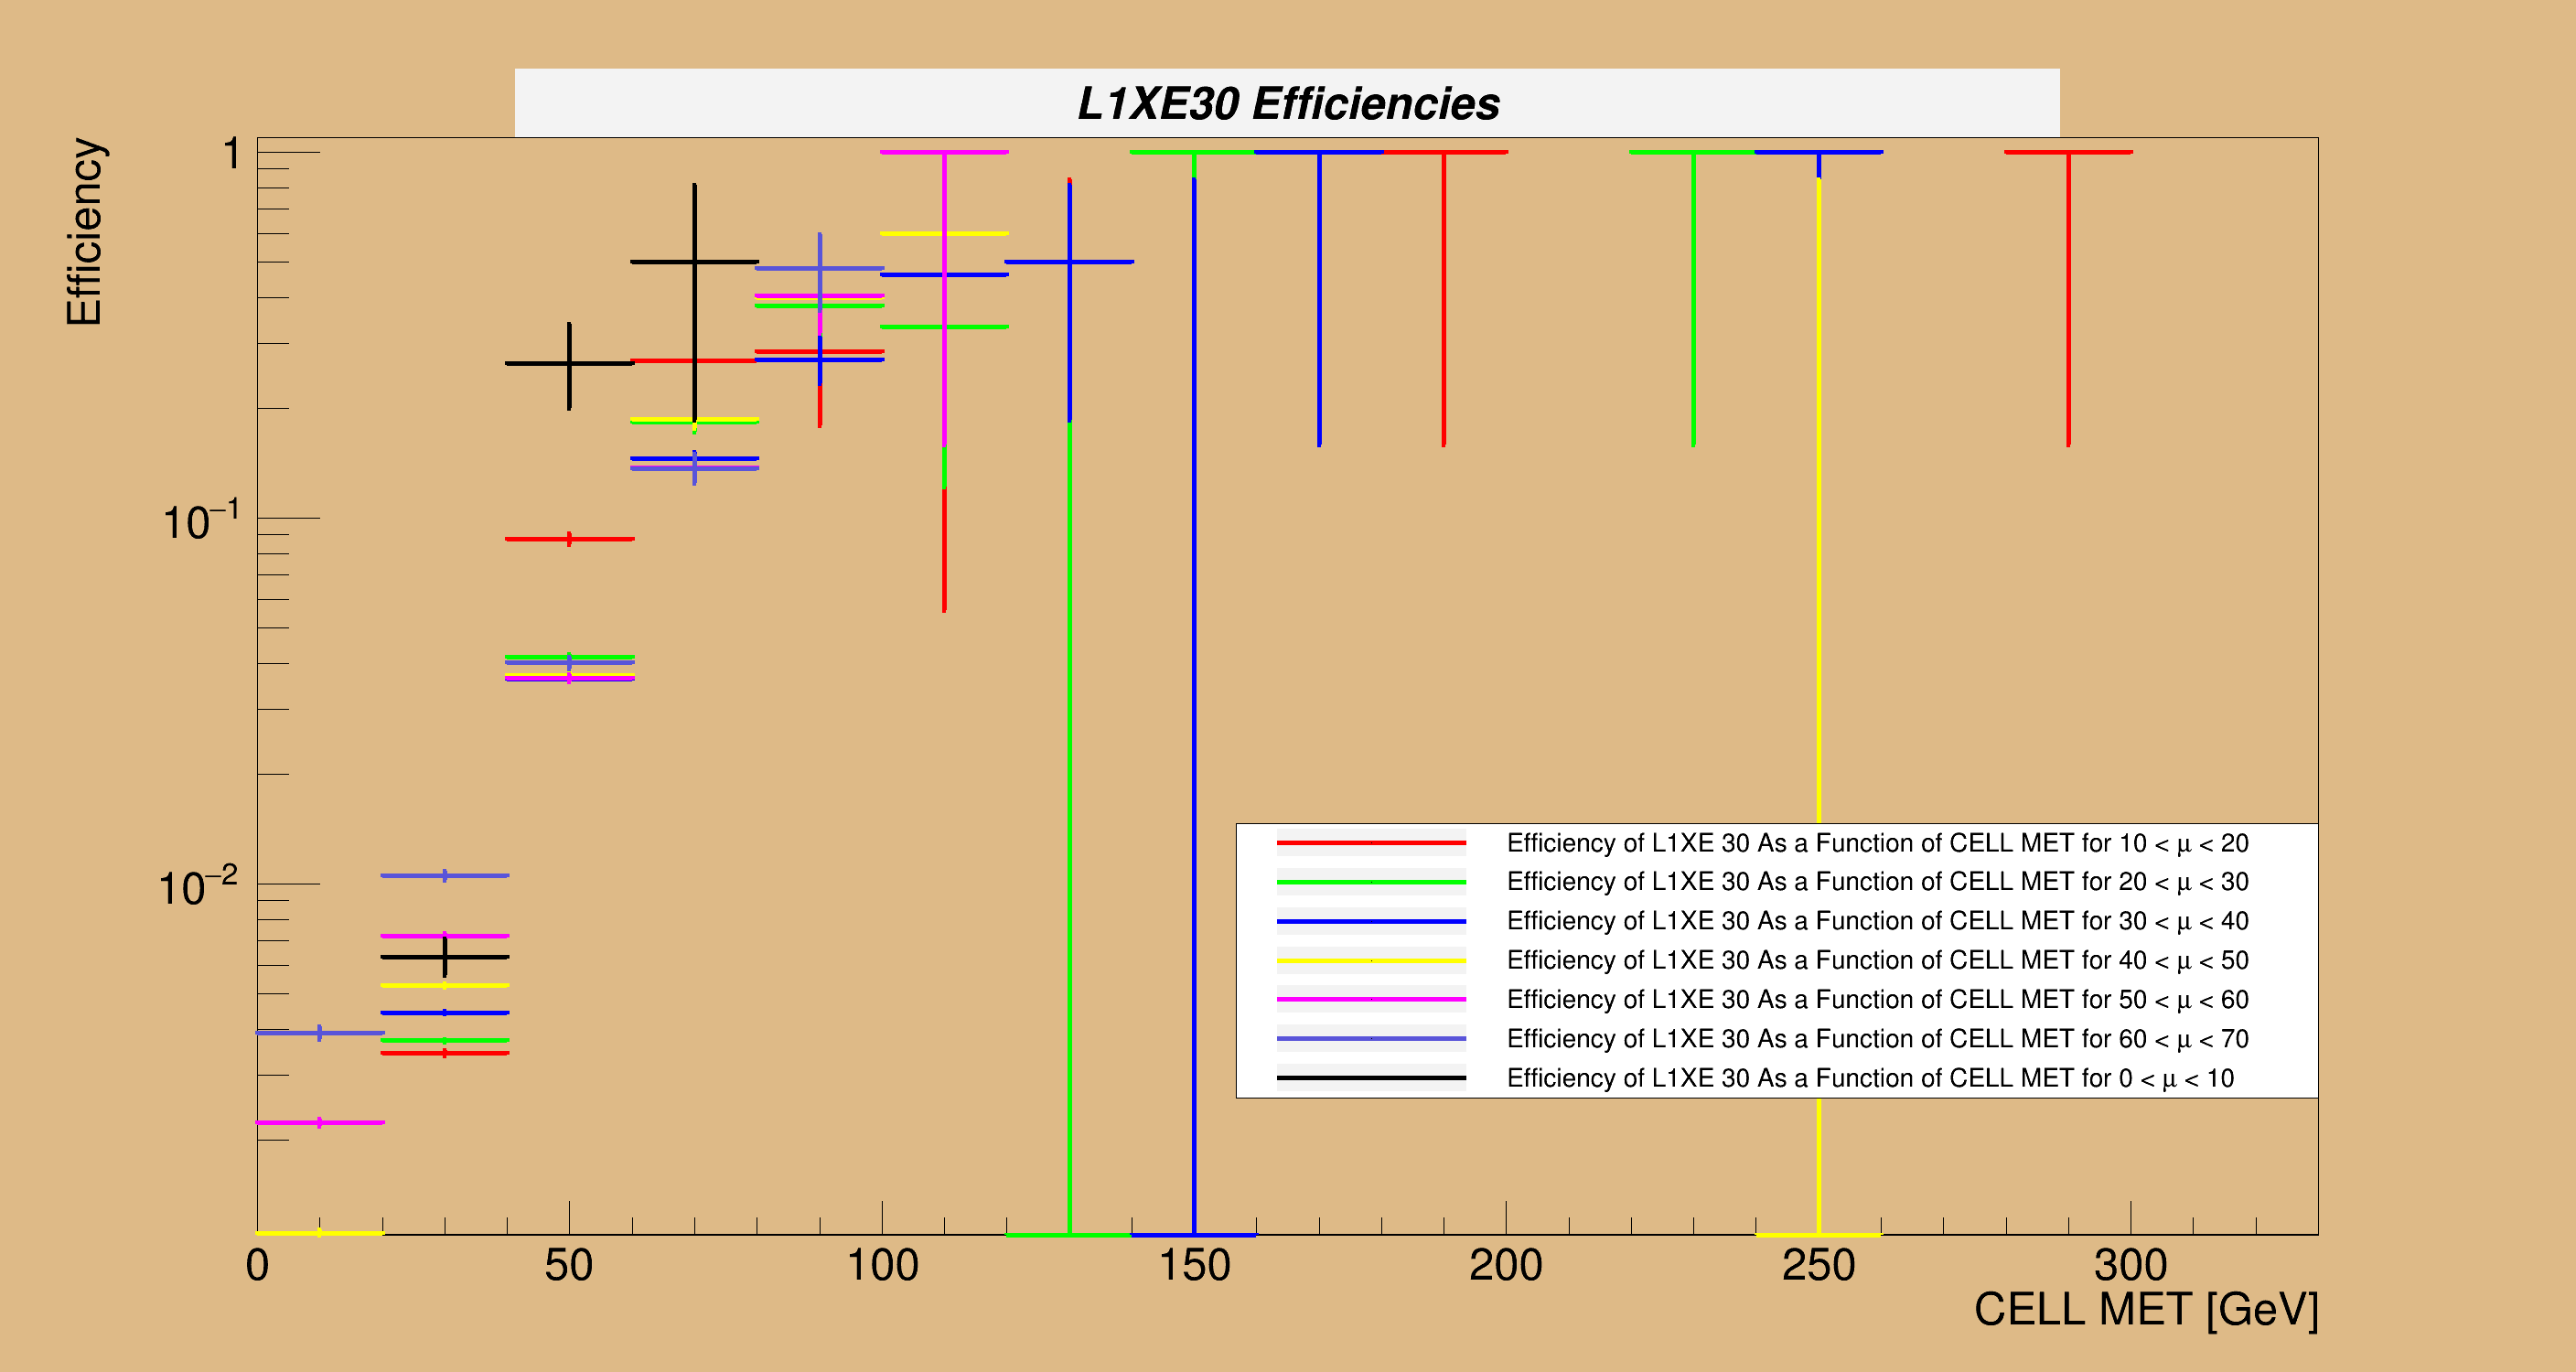
\includegraphics[scale=0.12]{L1XE30Efficiency_Curves}
		\caption{Efficiency Curves of L1$>30$ on the \texttt{HLT\_noalg\_L1ZB} data}
		%\label{fig:<+label+>}
\end{figure}
\begin{figure}[h]
		\centering
		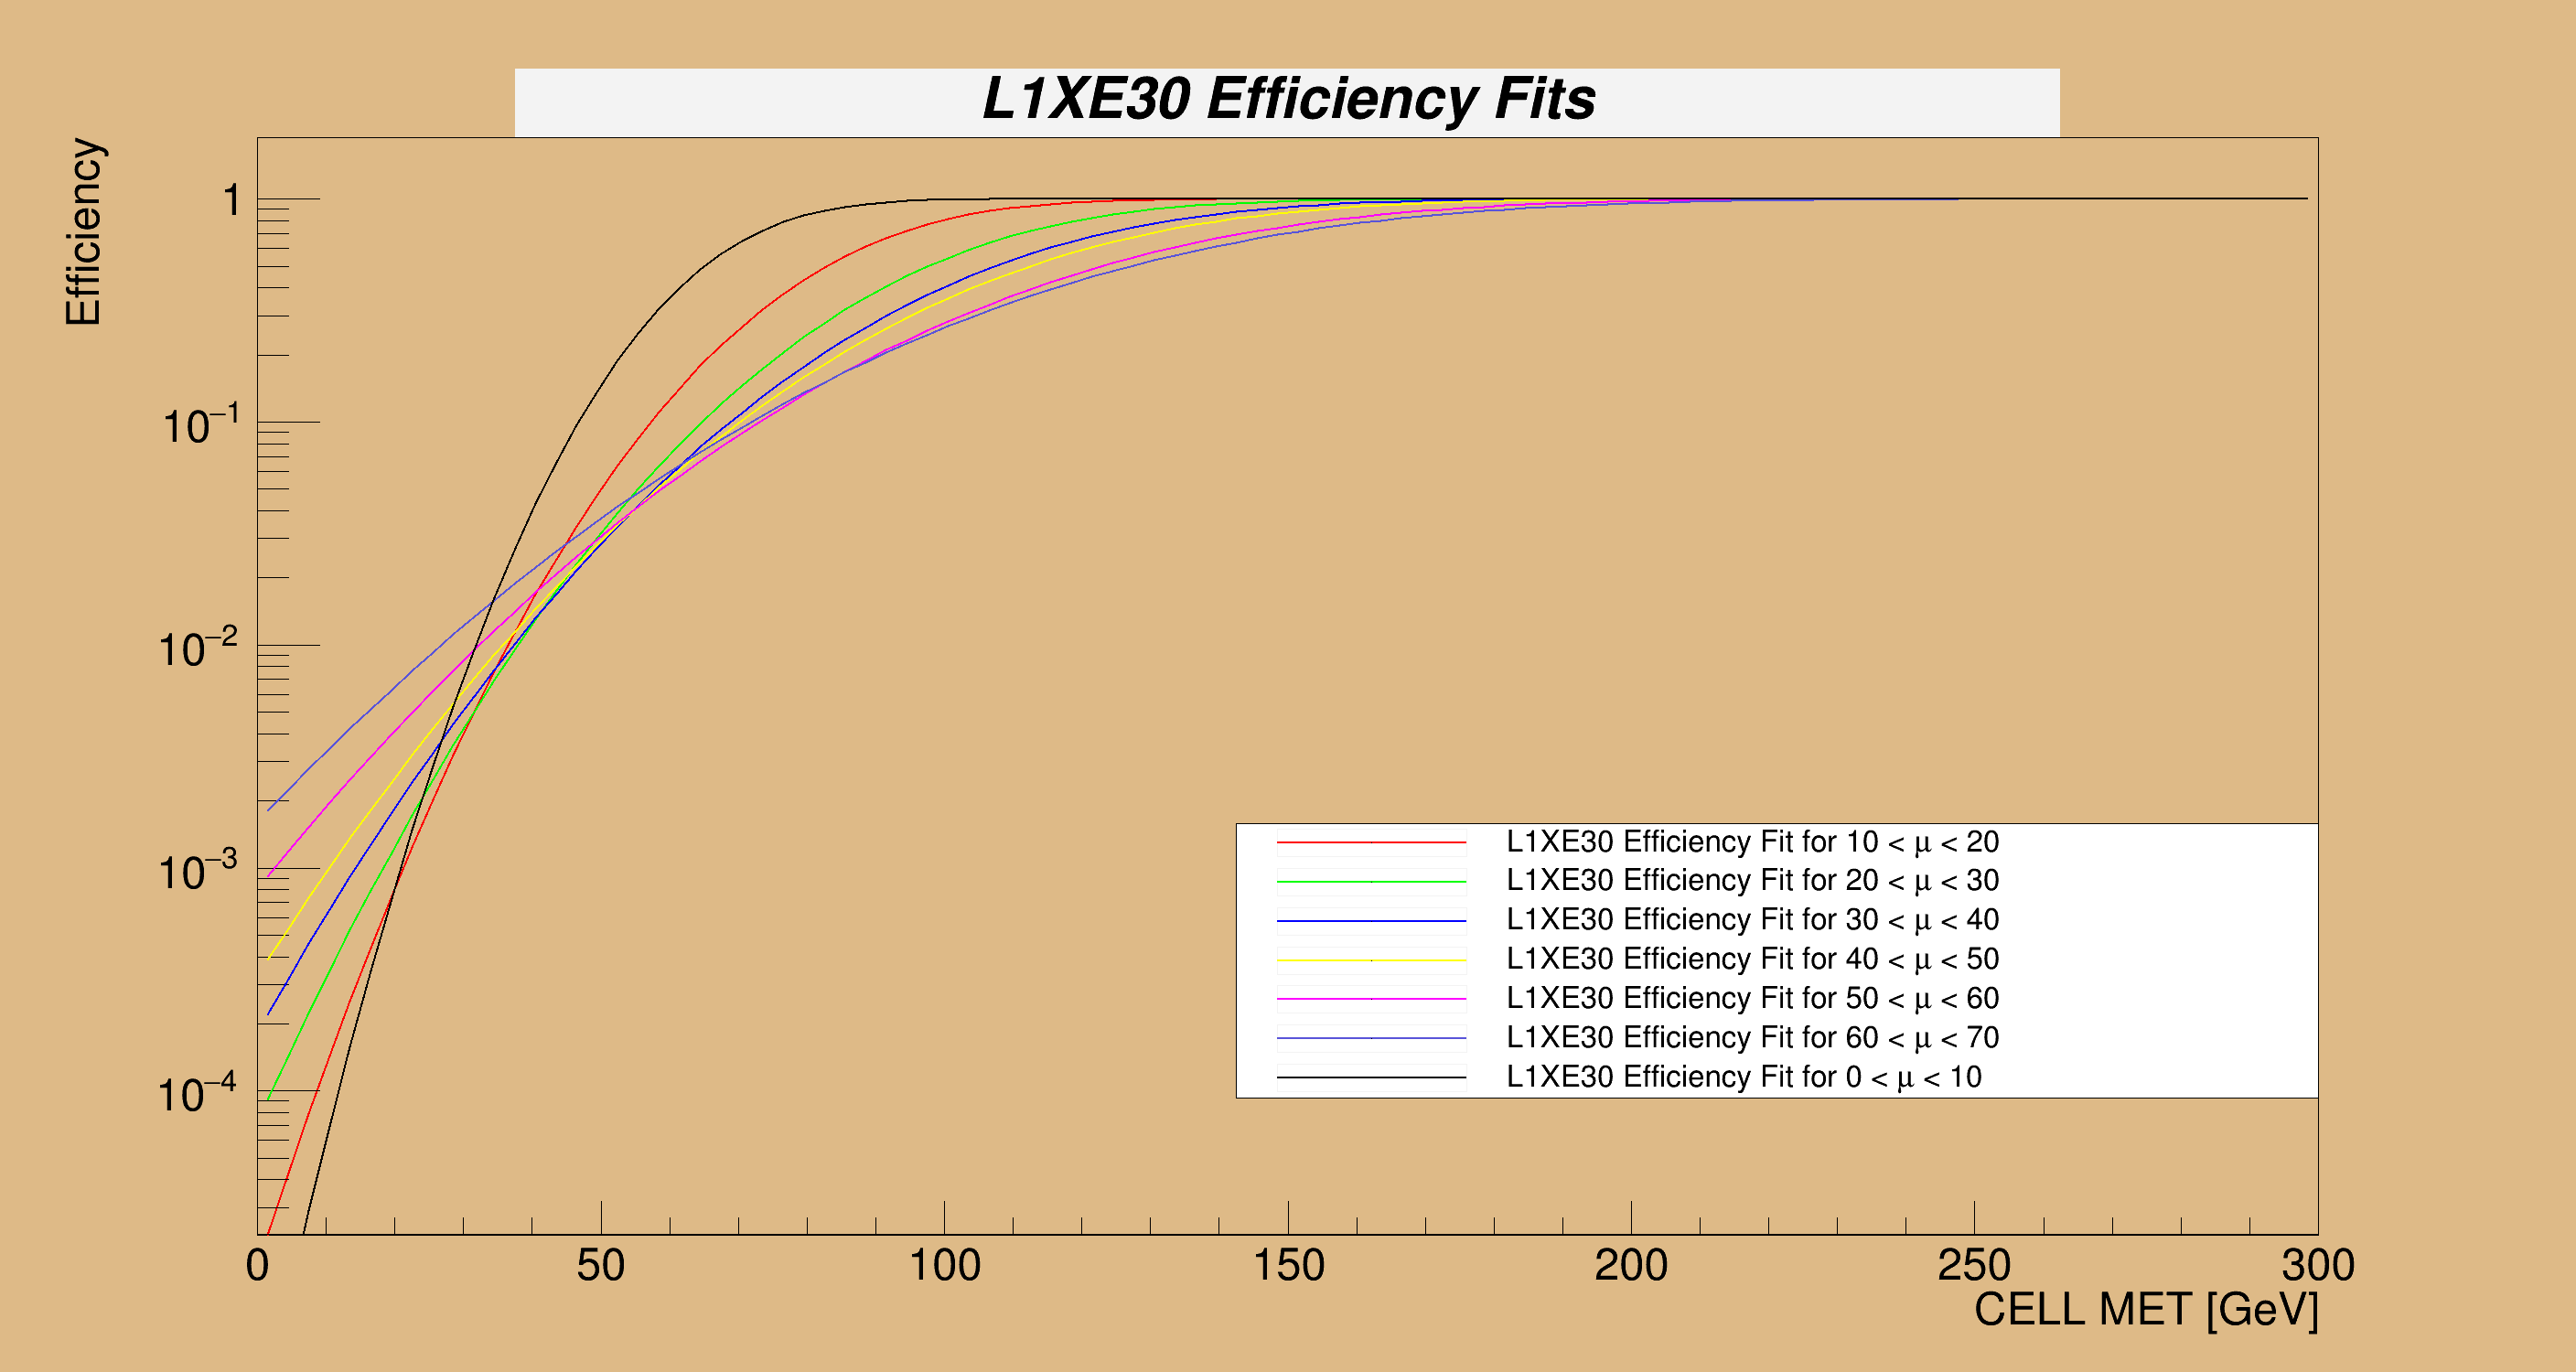
\includegraphics[scale=0.15]{L1XE30Efficiency_Fits}
		\caption{Efficiency Curves of L1$>30$ on the \texttt{HLT\_noalg\_L1ZB} data}
		%\label{fig:<+label+>}
\end{figure}
\begin{figure}[h]
		\centering
		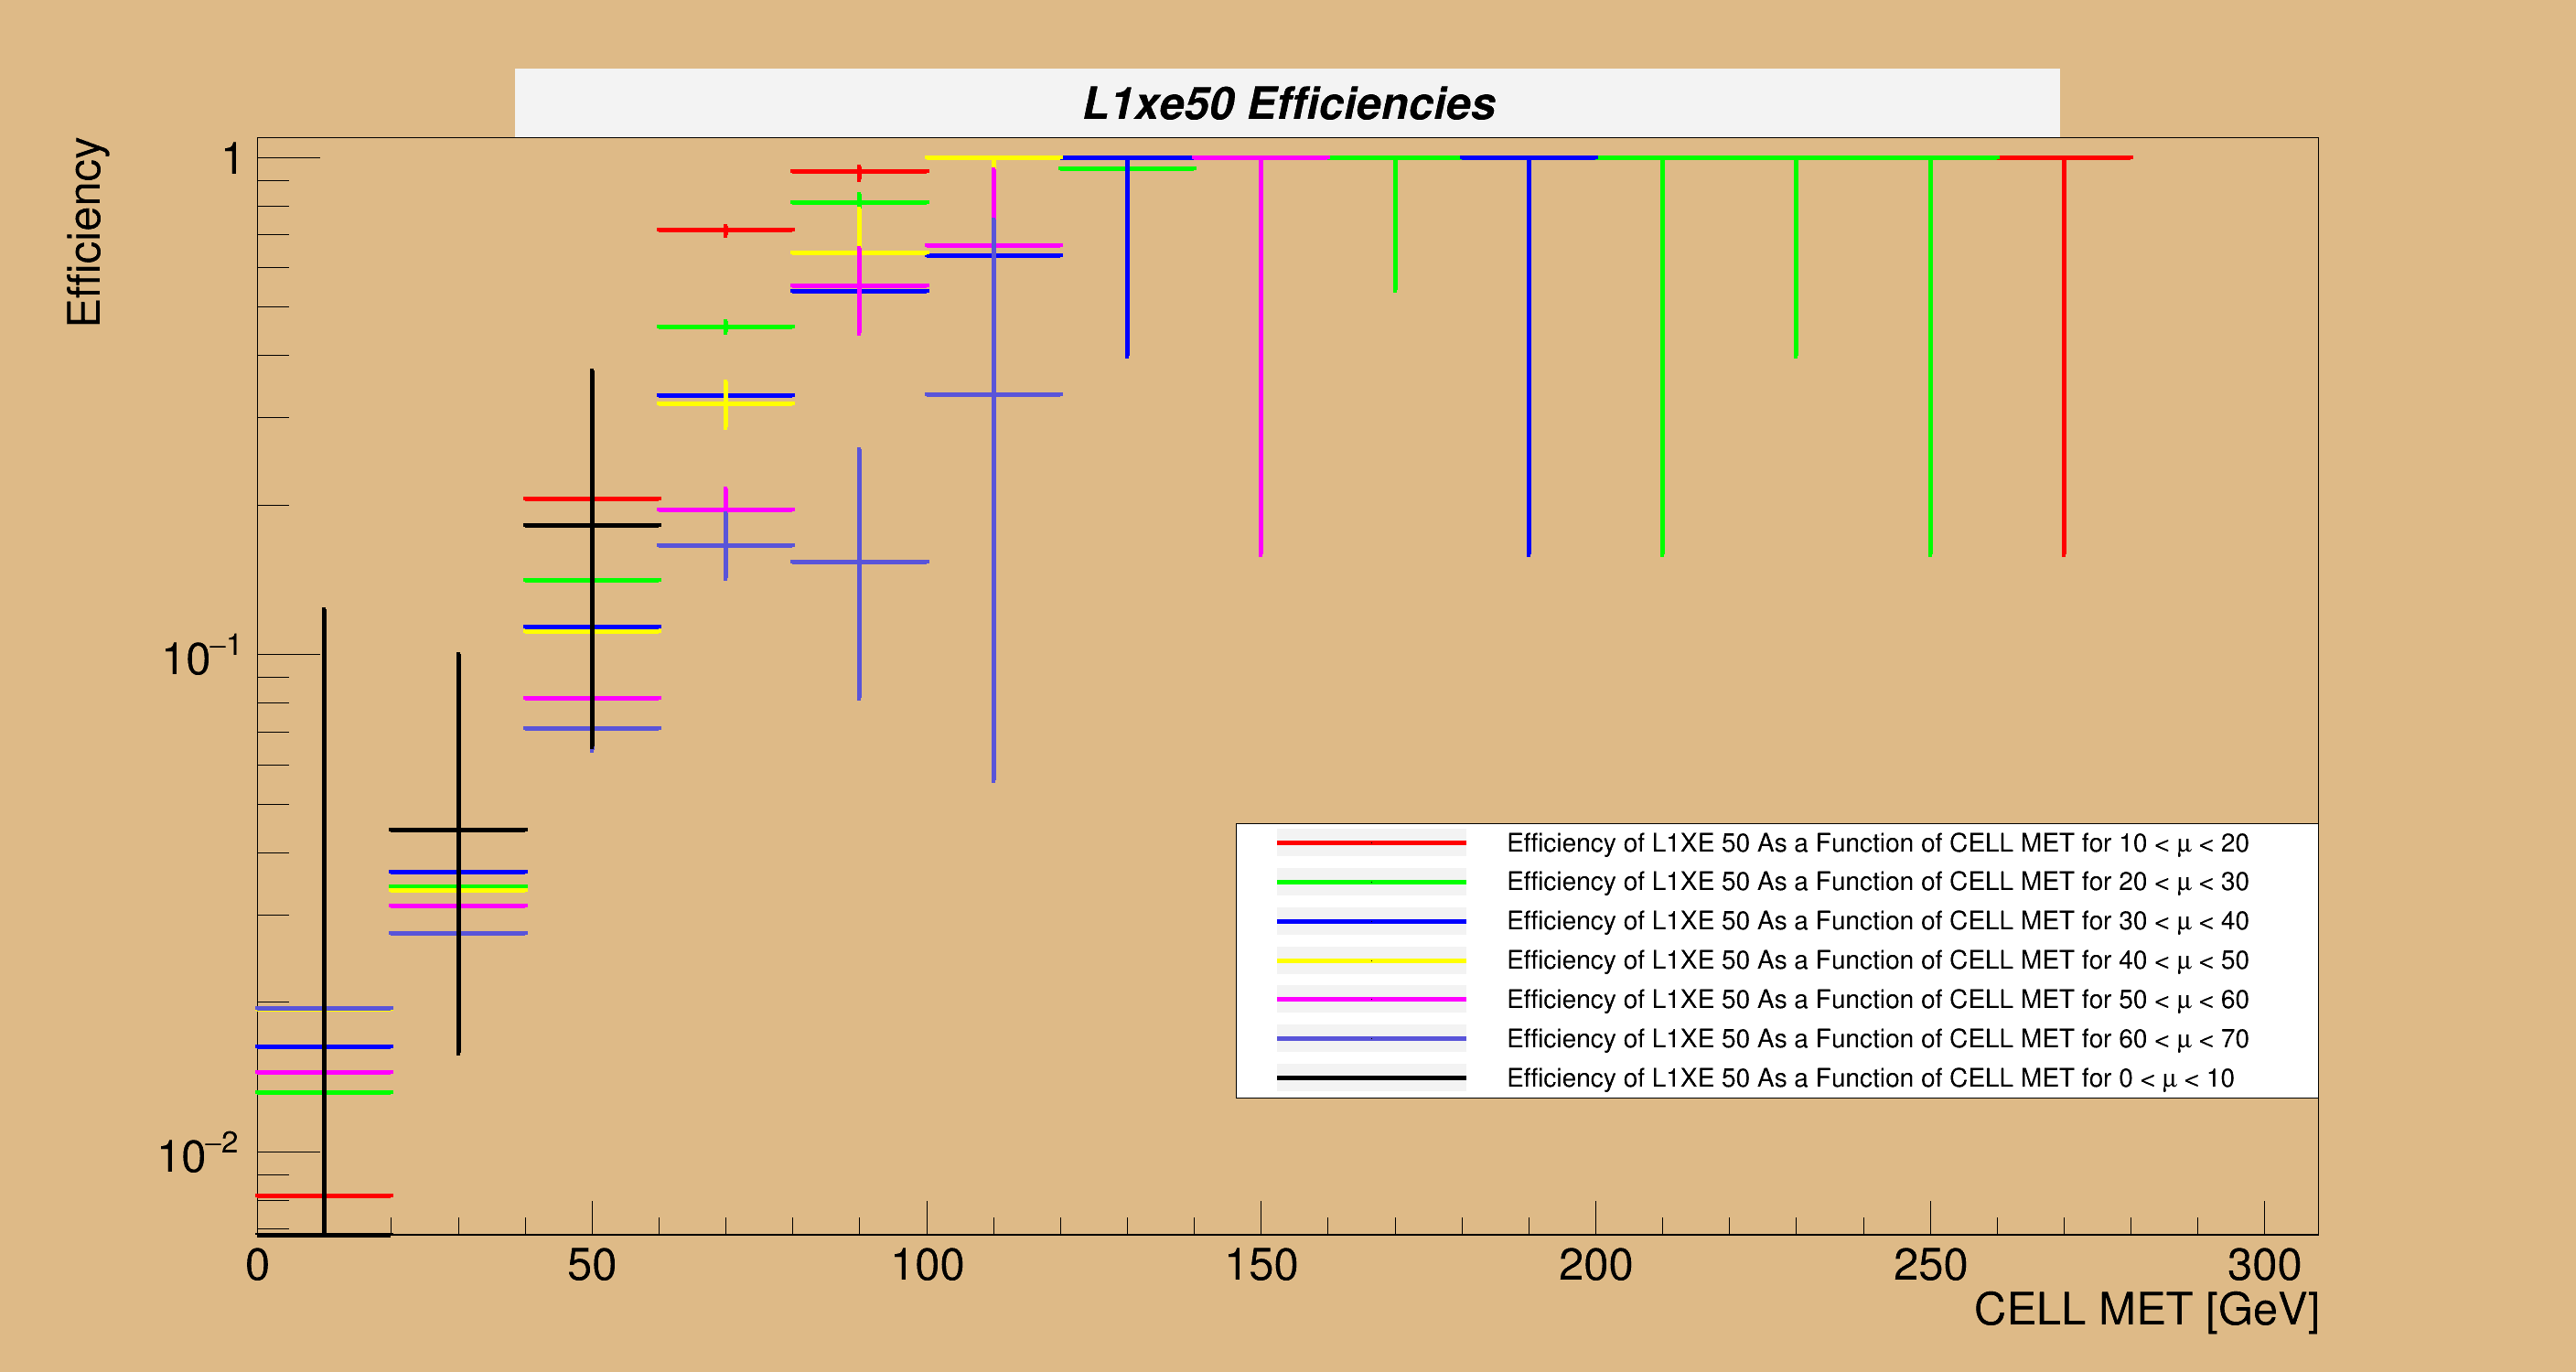
\includegraphics[scale=0.15]{L1XE50Efficiency_Curves}
		\caption{Efficiency Curves of L1$>50$ on the \texttt{HLT\_noalg\_L1XE30} data}
		%\label{fig:<+label+>}
\end{figure}
\begin{figure}[h]
		\centering
		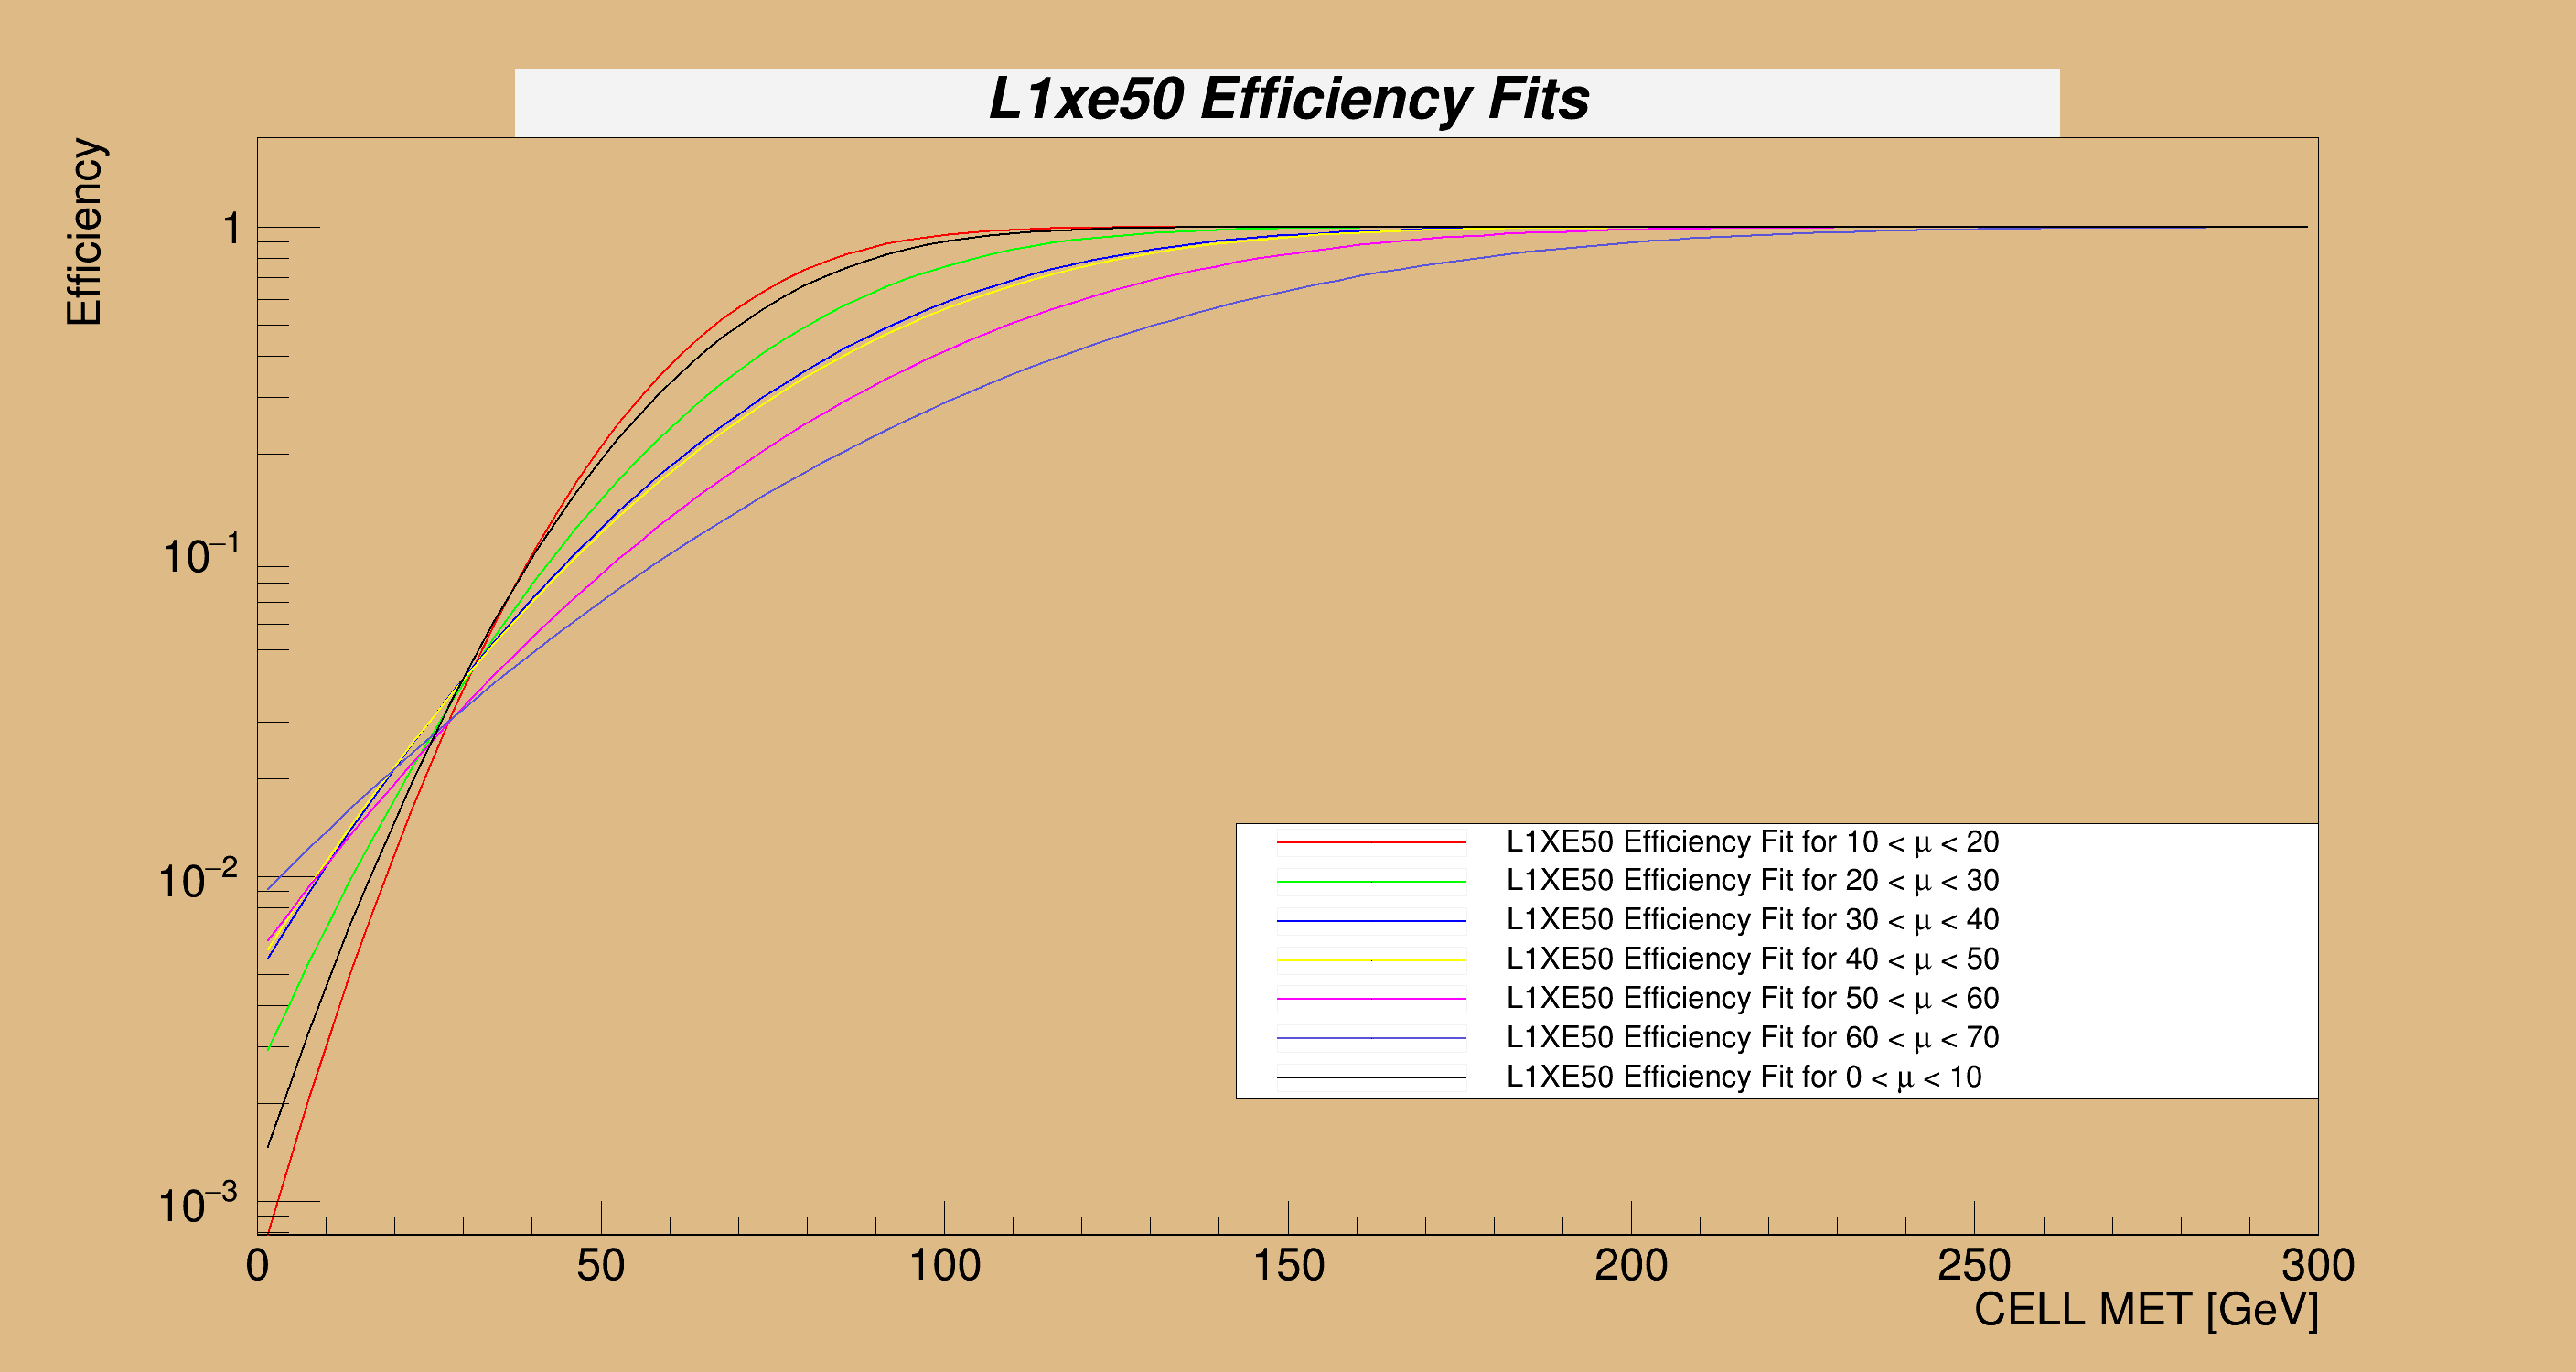
\includegraphics[scale=0.15]{L1XE50Efficiency_Fits}
		\caption{Efficiency Fits of L1$>50$ on the \texttt{HLT\_noalg\_L1XE30} data}
		%\label{fig:<+label+>}
\end{figure}
